\chapter{Baza}
\label{sec:robot}
\section{Dookólna platforma mobilna}
	\begin{figure}[H]
	\centering
	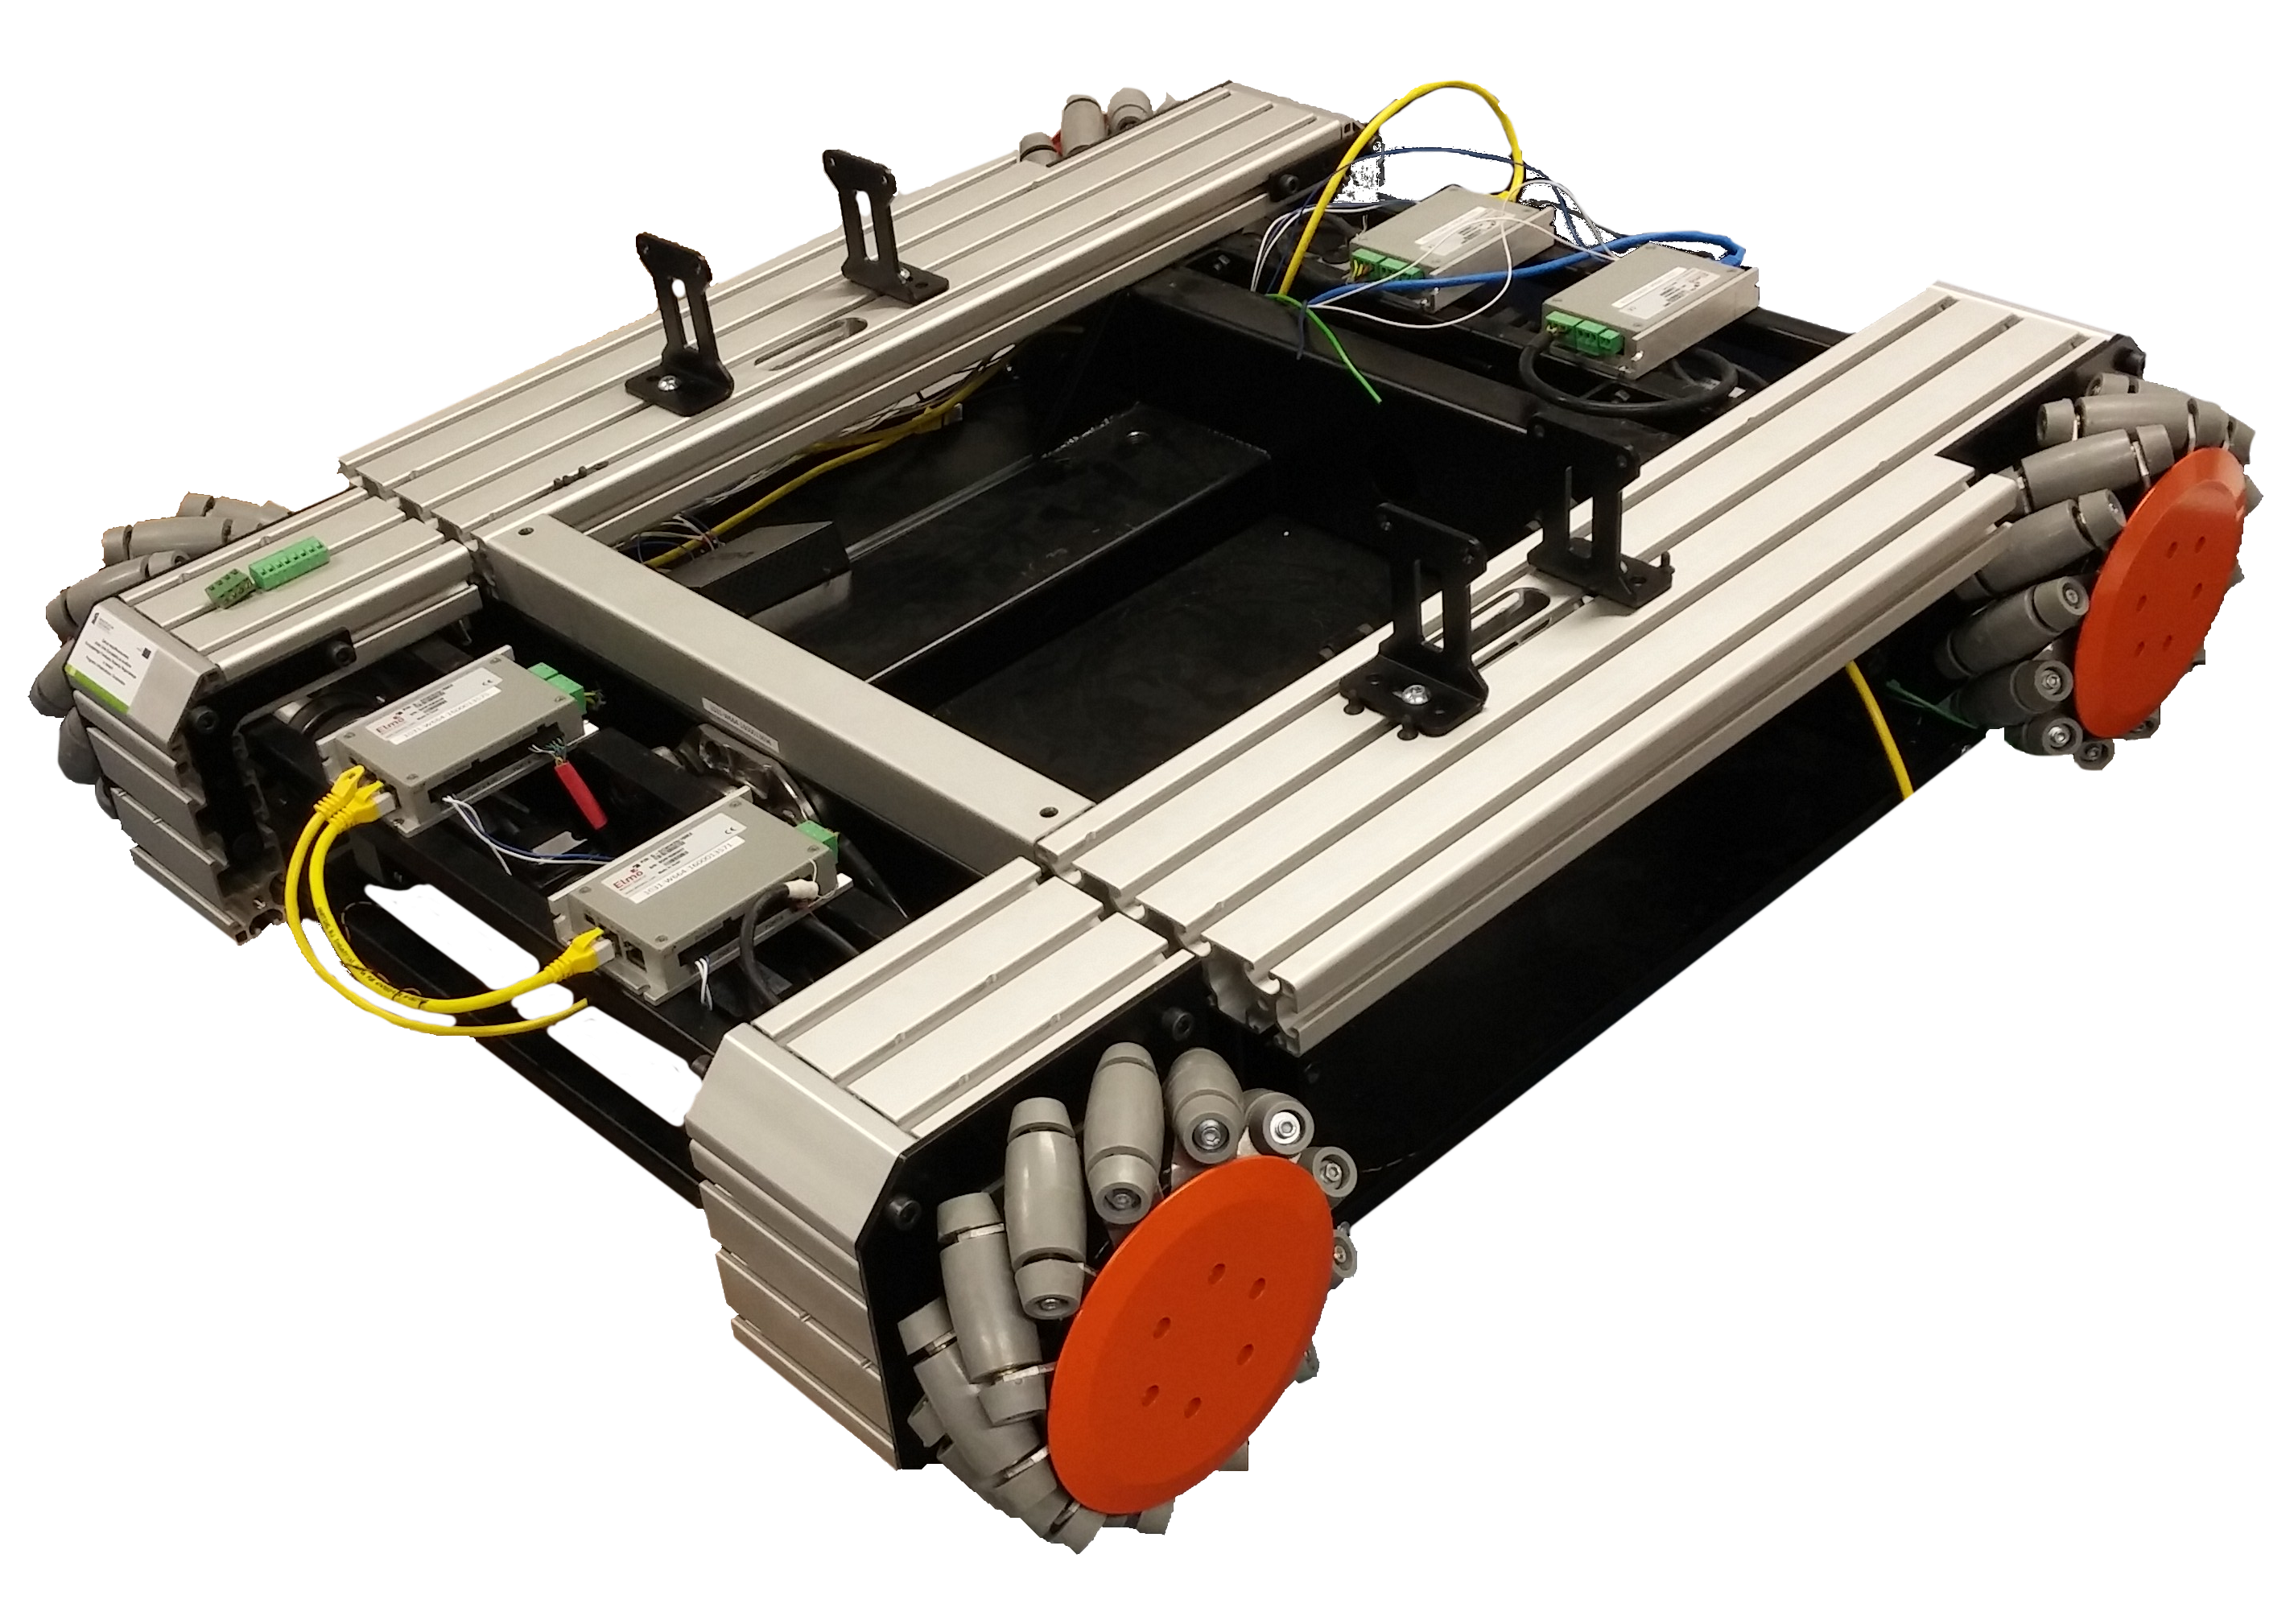
\includegraphics[width=0.8\textwidth]{graphics/base_photo.png}
	\caption{Dookólna baza mobilna na kołach szwedzkich.}
	\label{fig:base_photo}
	\end{figure} 

	Jest to duża, prostokątna baza dookólna, poruszająca się na czterech kołach szwedzkich, patrz fotografia \ref{fig:base_photo}.
	Koła są stałe, parami przytwierdzone do dwóch osi.
	Każde koło jest sterowane osobno przez podłączony bezpośrednio serwomotor, 
	zatem może mieć prędkość i kierunek niezależny od prędkości pozostałych kół, kierunku poruszania się robota, oraz jego obrotu.
	Każdy z serwomotorów ma także wbudowany enkoder.
	Sterownik enkodera zwraca aktualny kąt i prędkość obrotu.

	Jest to najpopularniejsza budowa dookólnych platform mobilnych, mająca zastosowanie także w innych robotach, jak na przykład Kuka Youbot \ref{fig:kuka_youbot}.
	Istnieją także roboty o trzech kołach szwedzkich, w których to koła rozstawione są promieniście pod kątami 120°.
	Pomimo prostszej budowy i takiej samej ilości stopni swobody, co czterokołowa wersja, stabilność takiego rozwiązania jest gorsza od zastosowanej tutaj budowy \cite{extra_axis}.
	Ponieważ jest to robot transportowy, to stabilność odgrywa tu ważną rolę i czterokołowa budowa jest wskazana.

	\begin{figure}[H]
	\centering
	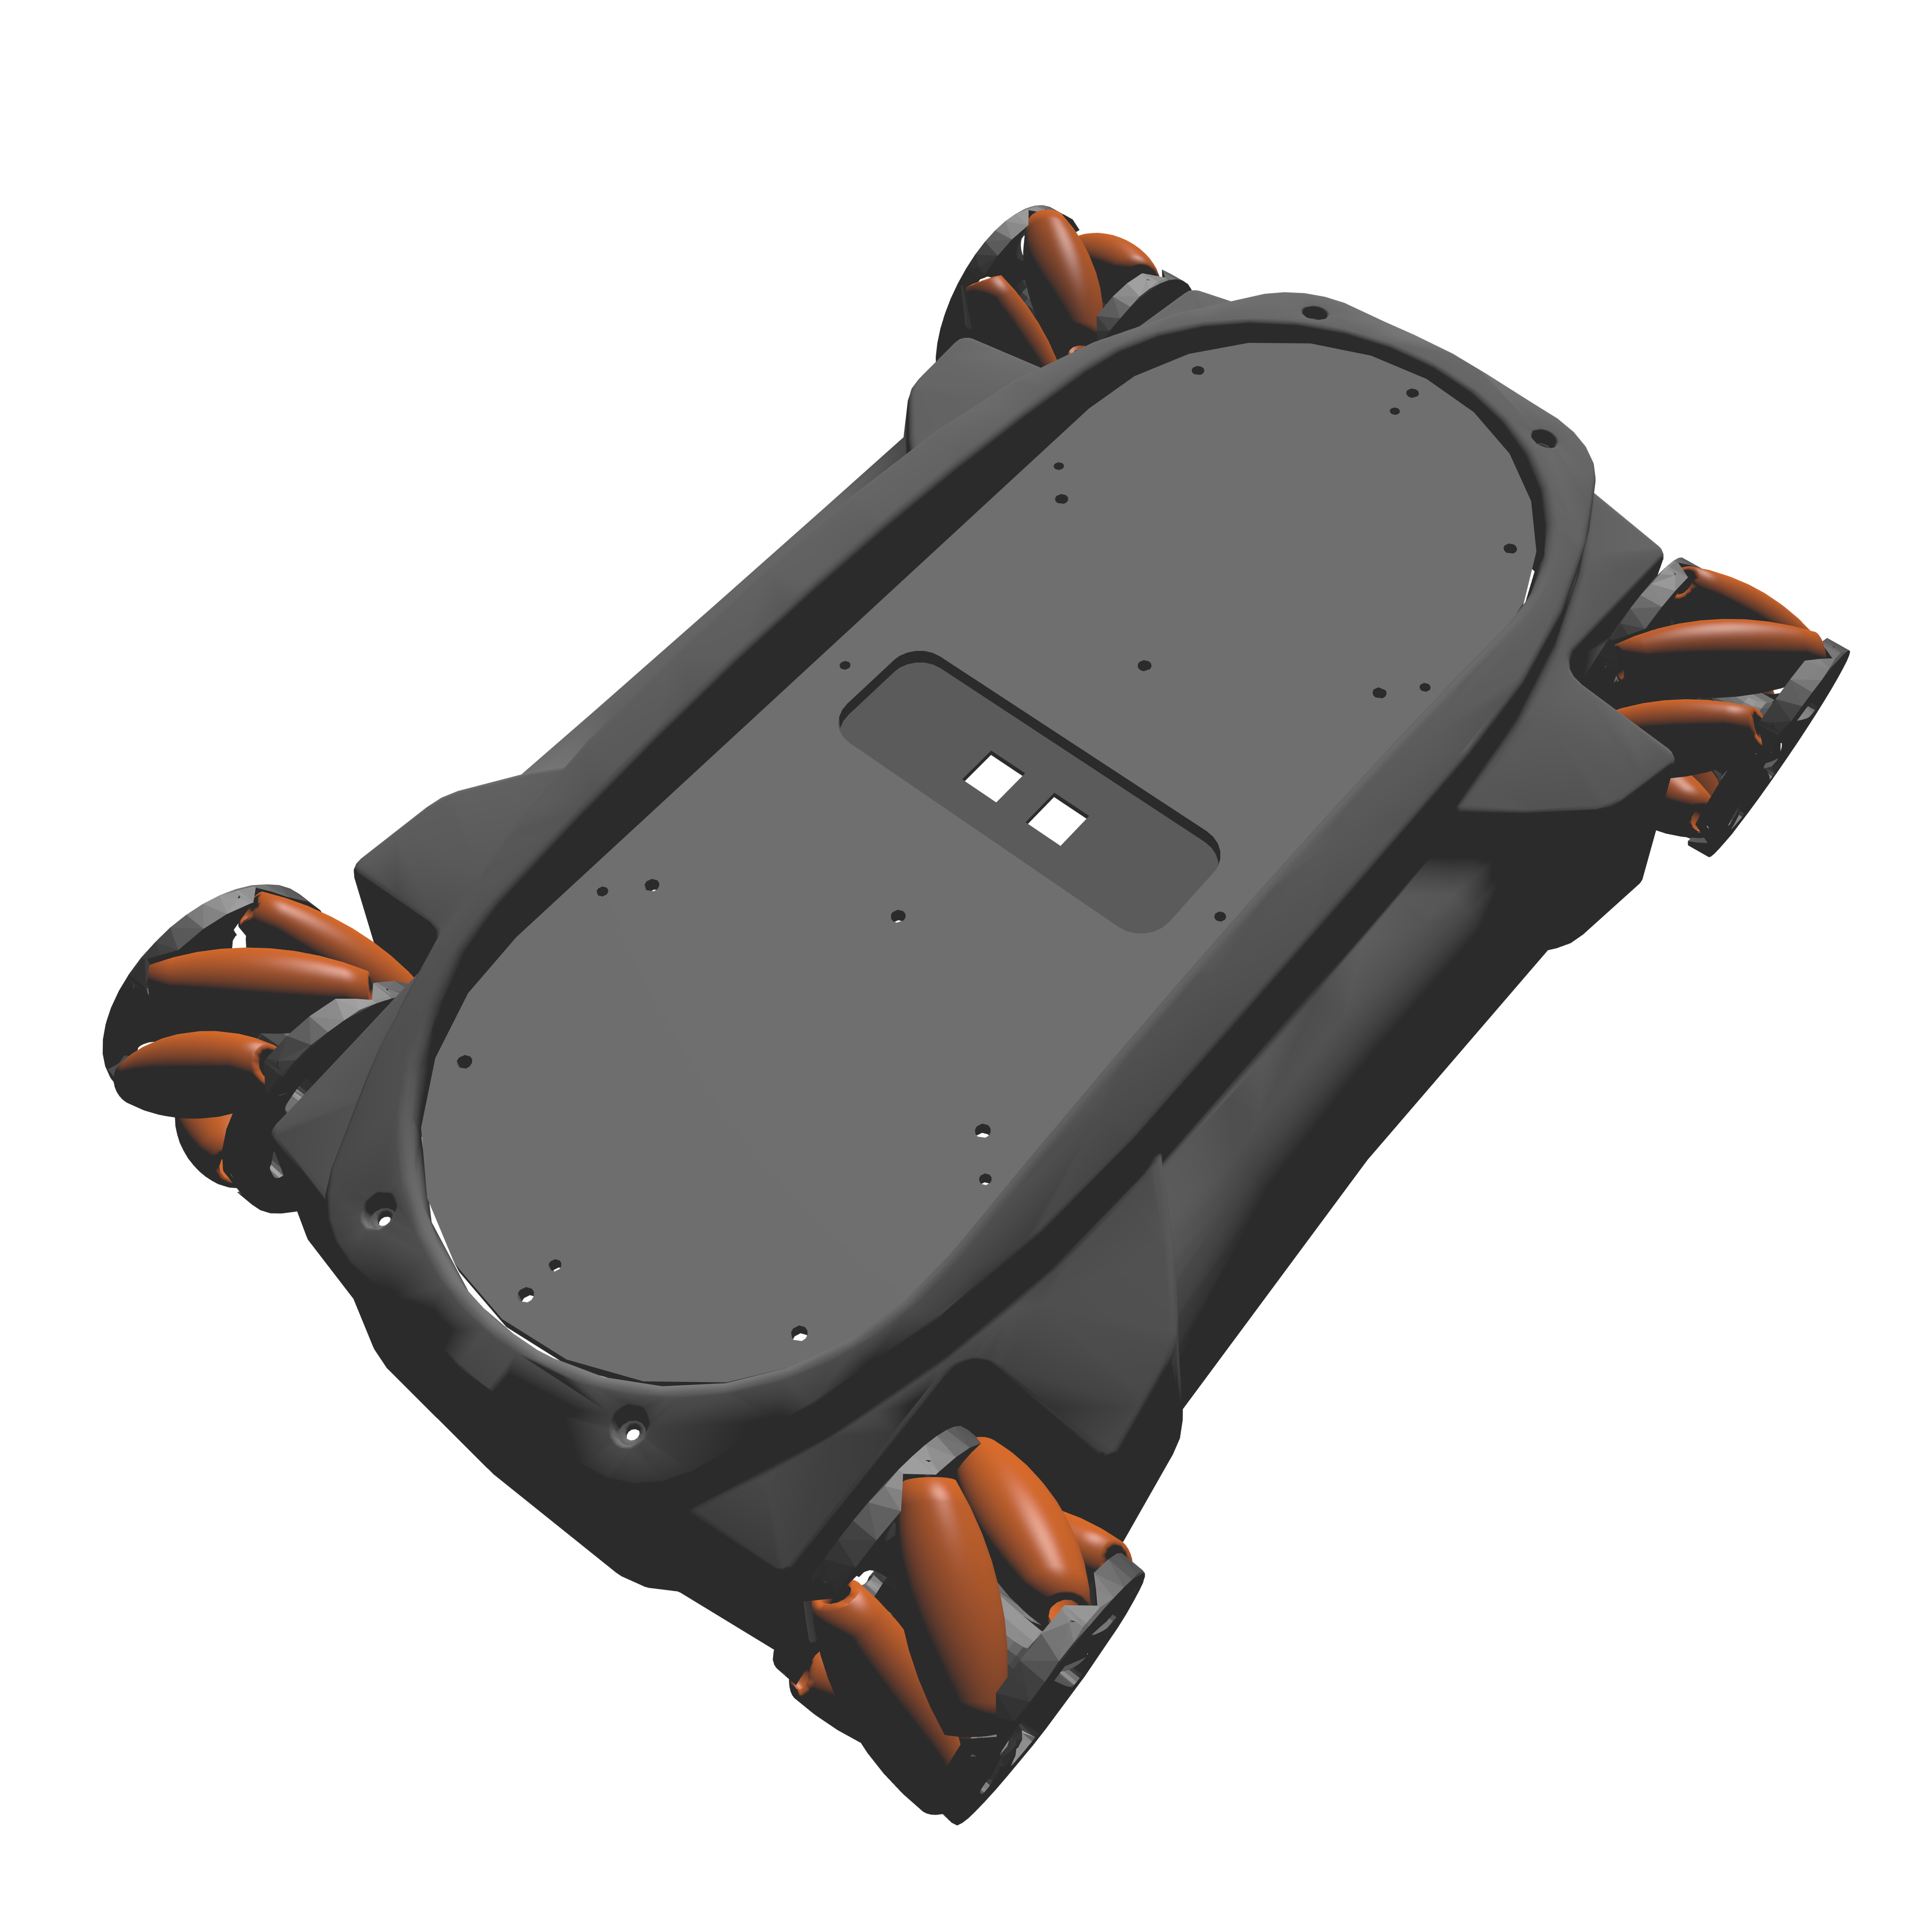
\includegraphics[width=0.5\textwidth]{graphics/kuka_youbot.png}
	\caption{Przykład innej platformy wielokierunkowej na podstawie fragmentu komercyjnego robota Kuka Youbot. 
	Należy zwrócić uwagę na charakterystyczne ustawienie kół, identyczne jak w opisywanej platformie \ref{fig:base_photo}.}
	\label{fig:kuka_youbot}
	\end{figure} 

	Odpowiedni obrót kół względem bazy, pozwala na jej ruch w dowolnym kierunku, niezależnym od kąta obrotu robota, patrz rysunek \ref{fig:mecanum_dirs}.
	Jest możliwe także obracać bazą, gdy ta porusza się w dowolnym kierunku, bądź stoi w miejscu.
	
	\begin{figure}[H]
	\centering
	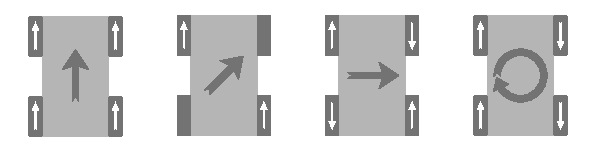
\includegraphics[width=0.8\textwidth]{graphics/mecanum_dirs.pdf}
	\caption{Podstawowe ruchy, jakie może wykonywać robot o napędzie wielokierunkowym.}
	\label{fig:mecanum_dirs}
	\end{figure} 
	
	Przykładowo, poruszając tylko przeciwległymi kołami po przekątnej, system będzie mógł poruszać po skosie, bez zmiany kąta obrotu.
	A jeśli do tego dodać obrót kół drugiej przekątnej, w odwrotnym kierunku, wtedy pojazd zacznie się poruszać w bok, pomimo faktu że koła nie są skrętne i 
	nie mogą ustawić się prosto do kierunku jazdy.
	Trasa po której porusza się robot, przy stałej prędkości kół, zawsze jest okręgiem, można uznać prostą za okrąg o nieskończonym promieniu, a punkt za okręg o zerowym.
	Wynika to z faktu, że każdy obiekt, który ma jednostajną prędkość i stały kierunek w lokalnym układzie współrzędnych, oraz prędkość kątową, będzie się poruszał po takiej krzywej.

	Podstawa ma za zadanie transportować robota manipulującego Velma, tworząc razem manipulator mobilny.
	Velma to wysoki i bardzo ciężki robot, wyposażony w dwa chwytaki na ramionach o wielu przegubach, patrz fotografia \ref{fig:velma}.
	Taka budowa wymaga szerokiej podstawy, aby zachować bezpieczną równowagę całości.
	Jeżdżąc na tej podstawie, robot może się przemieszczać i obracać w dowolnym kierunku, aby uzyskać lepszy dostęp do manipulowanych przedmiotów.
	Dodatkowe czujniki laserowe umieszczone tuż nad postawą odpowiadają za wykrywanie kolizji i lokalizację.

	\begin{figure}[H]
	\centering
	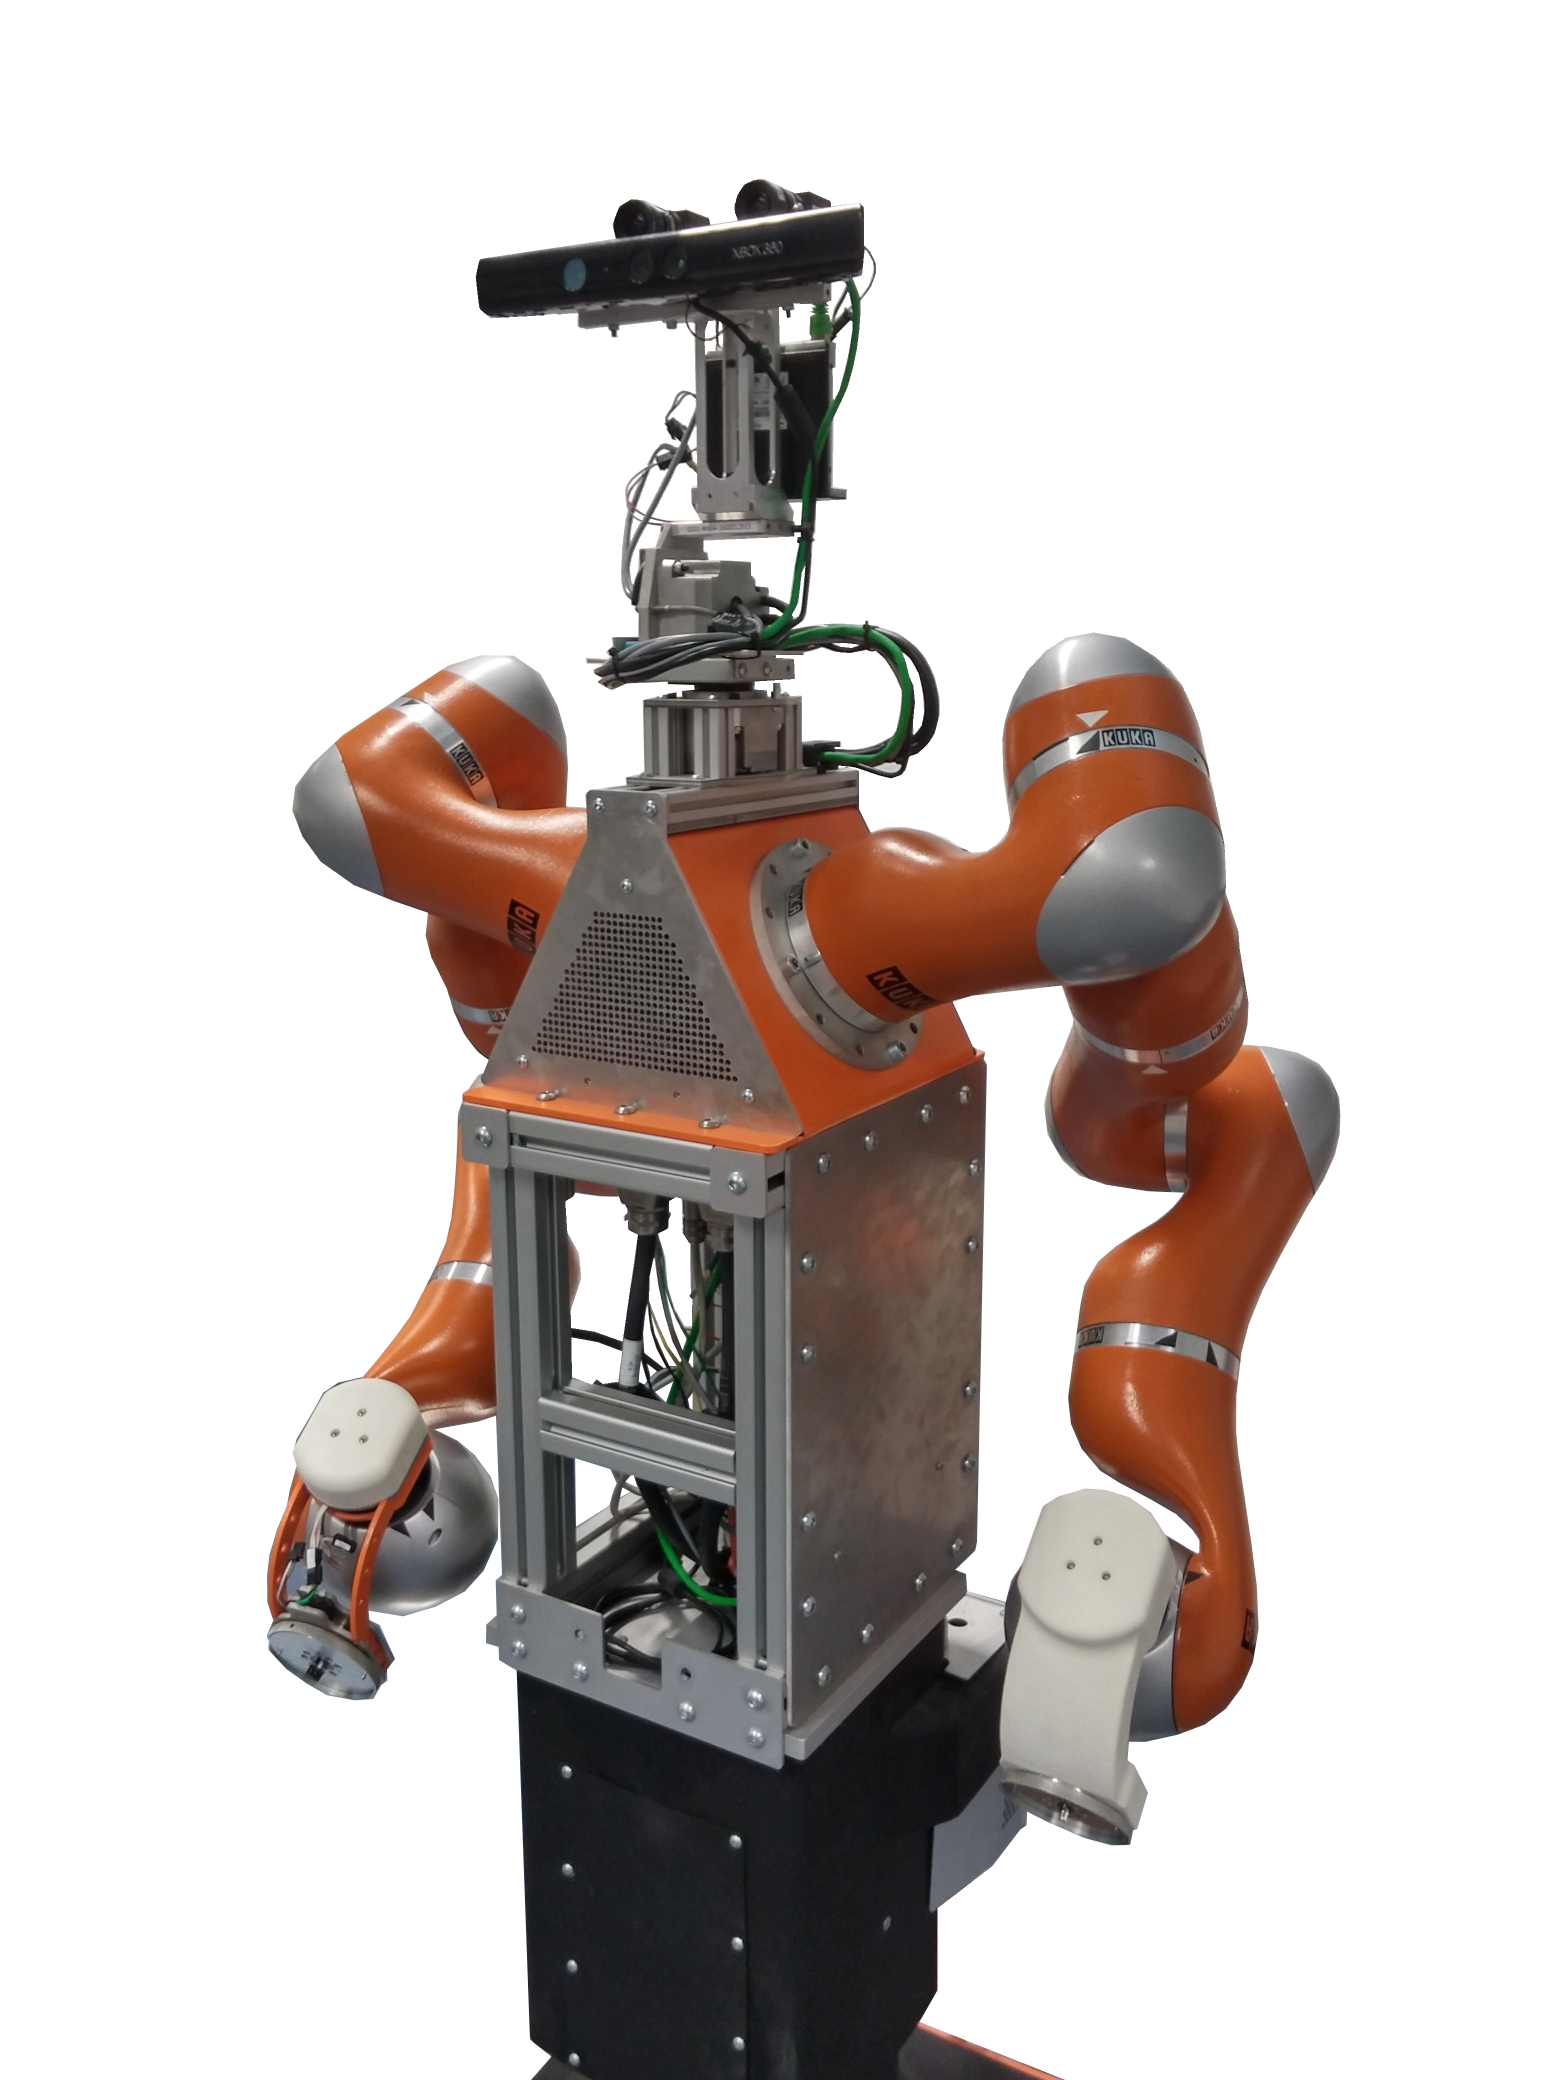
\includegraphics[width=0.5\textwidth]{graphics/velma.png}
	\caption{Robot manipulacyjny Velma.}
	\label{fig:velma}
	\end{figure} 

	Platforma jest niesymetrycznie podzielona na dwie niezależne części, przednią i tylną, w sposób pokazany na rysunku \ref{fig:base_top}.
	Przegub o jednym stopniu swobody (tzw. zawias) jest jedynym łącznikiem pomiędzy tymi dwoma fragmentami.
	Zadaniem tego przegubu jest zmniejszanie wpływu nierówności podłoża na ruch bazy, aby każde koło dociskało do podłoża z taką samą siłą, jak po drugiej stronie osi.
	Bez tego zawiasu nierówny teren uniemożliwiałby sprawne sterowanie platformą na skutek niedeterministycznego tarcia kół tej samej osi, powodując nieplanowany skręt.
	Niedeterministyczne tarcie kół jest niewykrywalne w bezpośredni sposób, jak to zostało opisane w \cite{boringbot}.

	Platforma nie jest idealnym kwadratem, jest 4 cm różnicy między szerokością, a długością robota.
	Także środki kół nie są ustawione na wierzchołkach tej figury geometrycznej.
	Szerokość jest większa, co można zobaczyć porównując widok z prawej strony \ref{fig:base_side} z widokiem z tyłu \ref{fig:base_front}.
	Dokładne wymiary są podane na rysunku \ref{fig:base_dims} i tabeli \ref{tab:dims}.

	Platforma podatna jest na losowy ruch przy rozpoczynaniu jazdy i hamowaniu.
	Jest to spowodowane tym, że asymetria rolek będzie nadawać kołom różne siły oporu, a w związku z tym różne prędkości, co w efekcie może powodować niedeterministyczny ruch.
	Należy także wziąć tutaj pod uwagę inne cechy budowy kół, jak nierówne tarcie rolek o powierzchnię \cite{braking}.

	\begin{figure}[H]
	\centering
	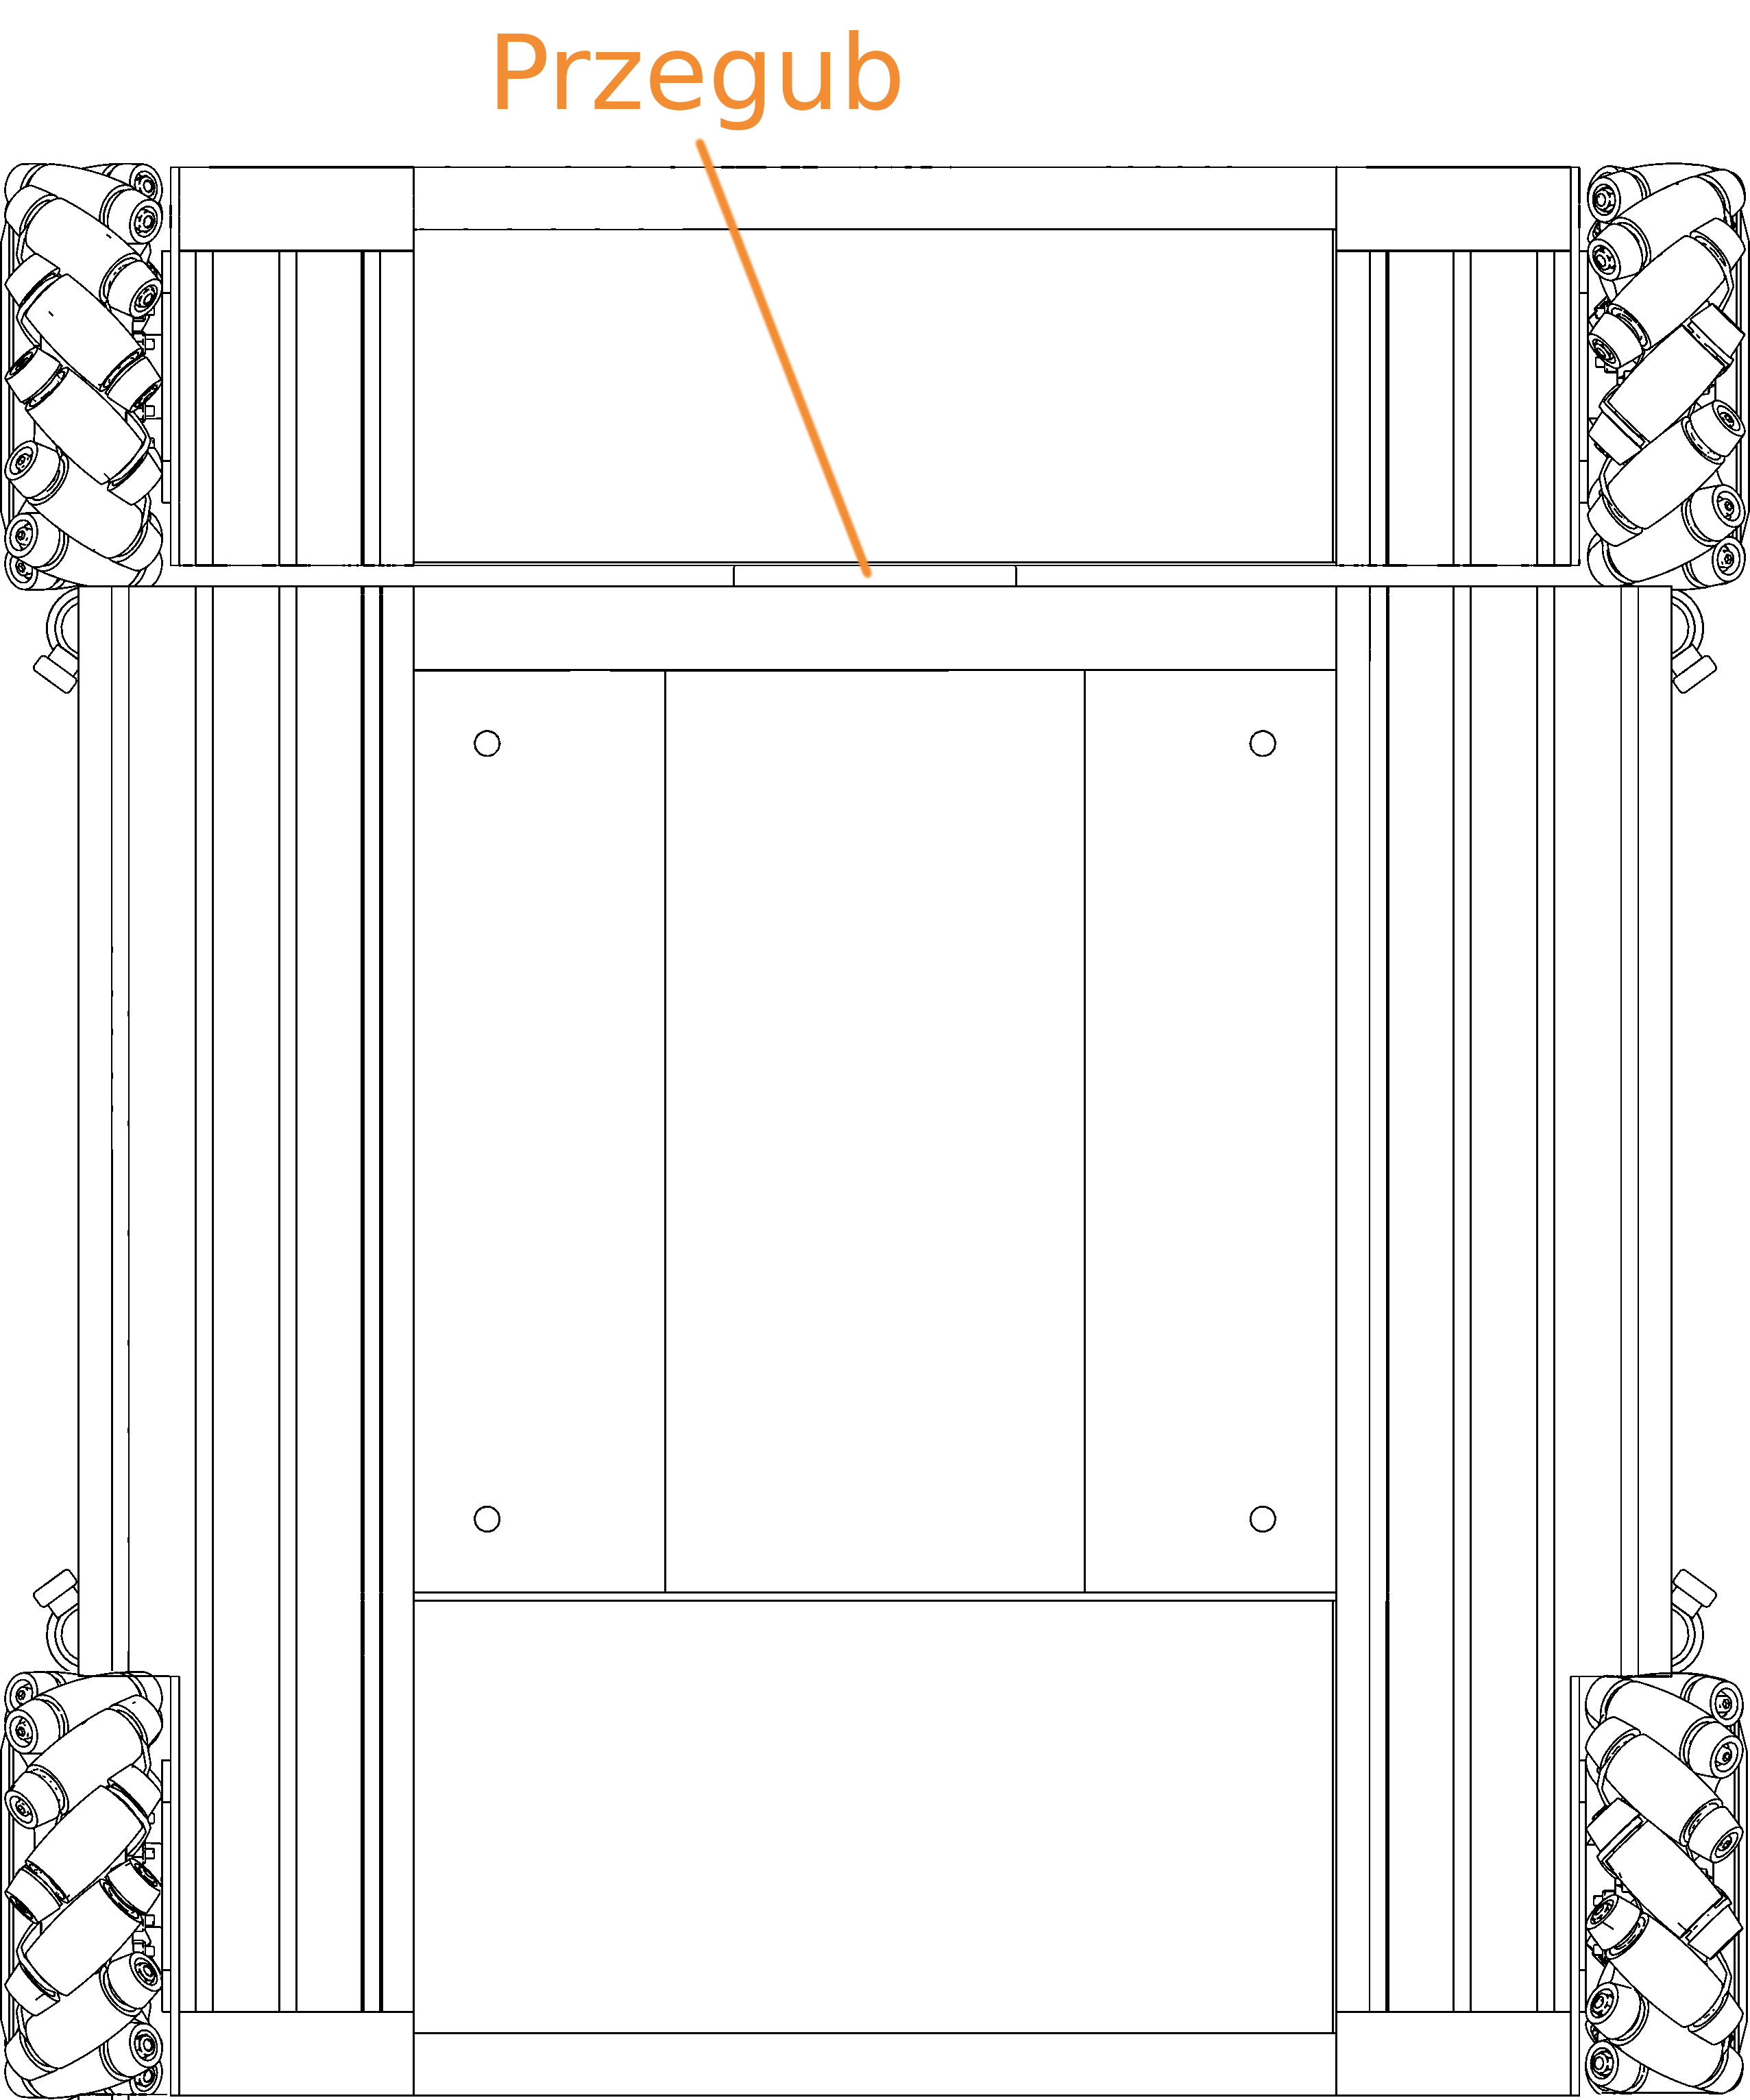
\includegraphics[width=0.5\textwidth]{graphics/base_top.png}
	\caption{Platforma mobilna --- widok od góry. Przegub zawiasowy łączy dwie części.}
	\label{fig:base_top}
	\end{figure} 

	\begin{figure}[H]
	\centering
	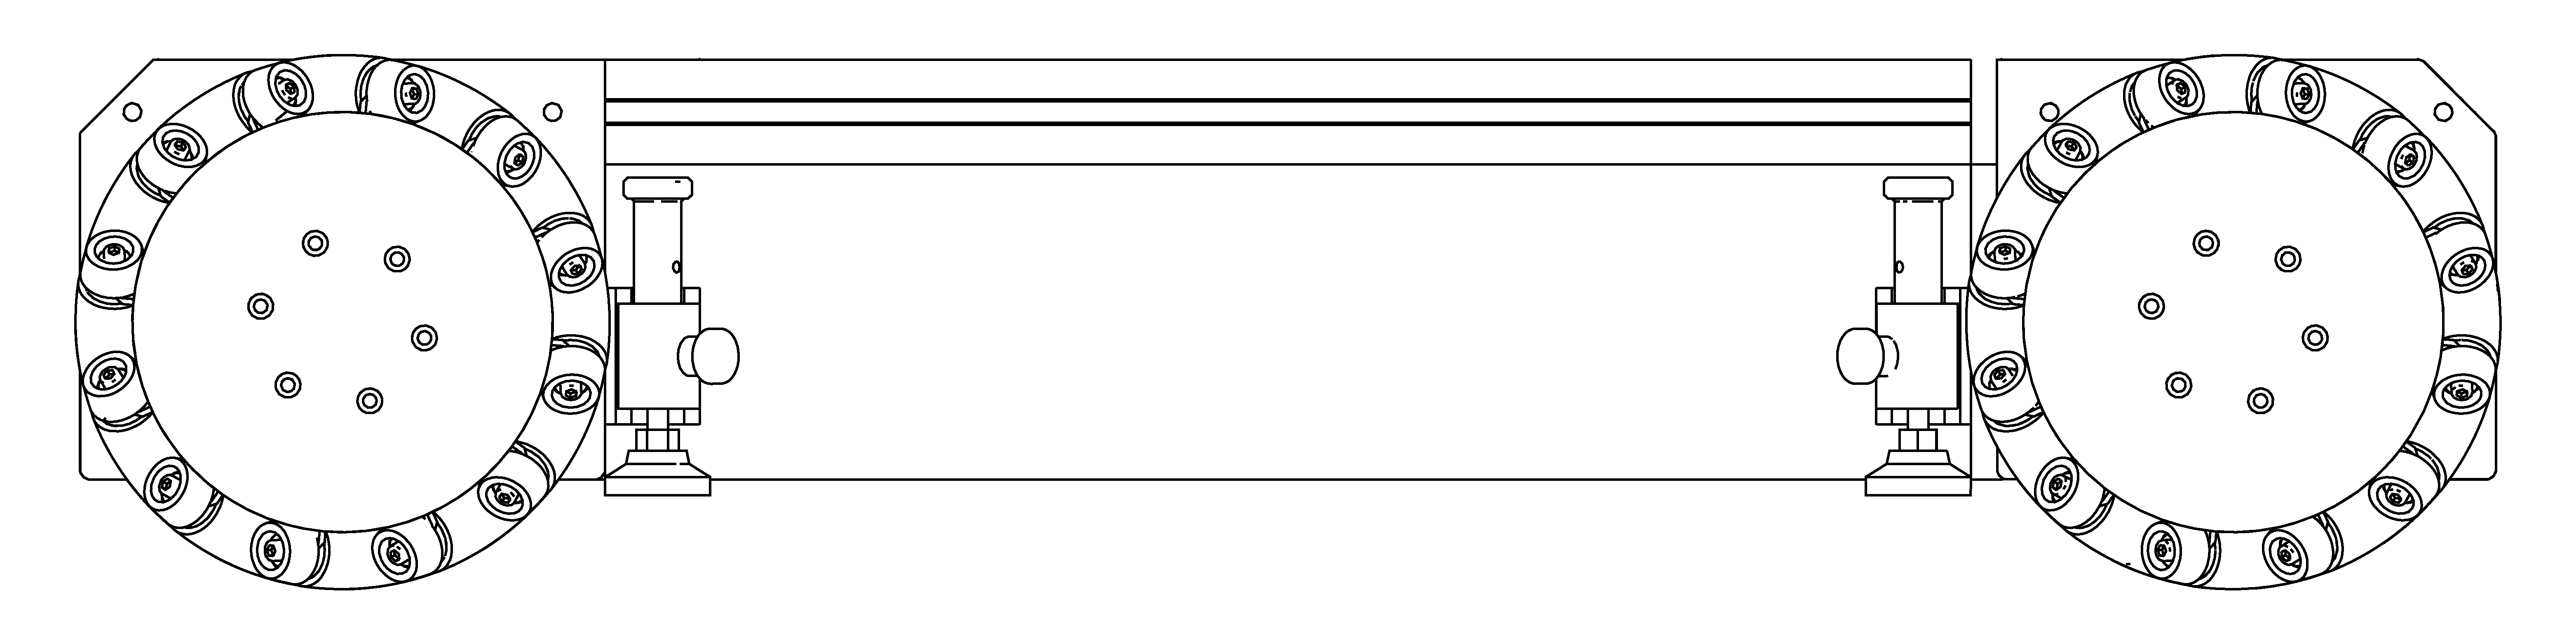
\includegraphics[width=0.5\textwidth]{graphics/base_side.pdf}
	\caption{Platforma mobilna --- widok z prawej strony.}
	\label{fig:base_side}
	\end{figure} 

	\begin{figure}[H]
	\centering
	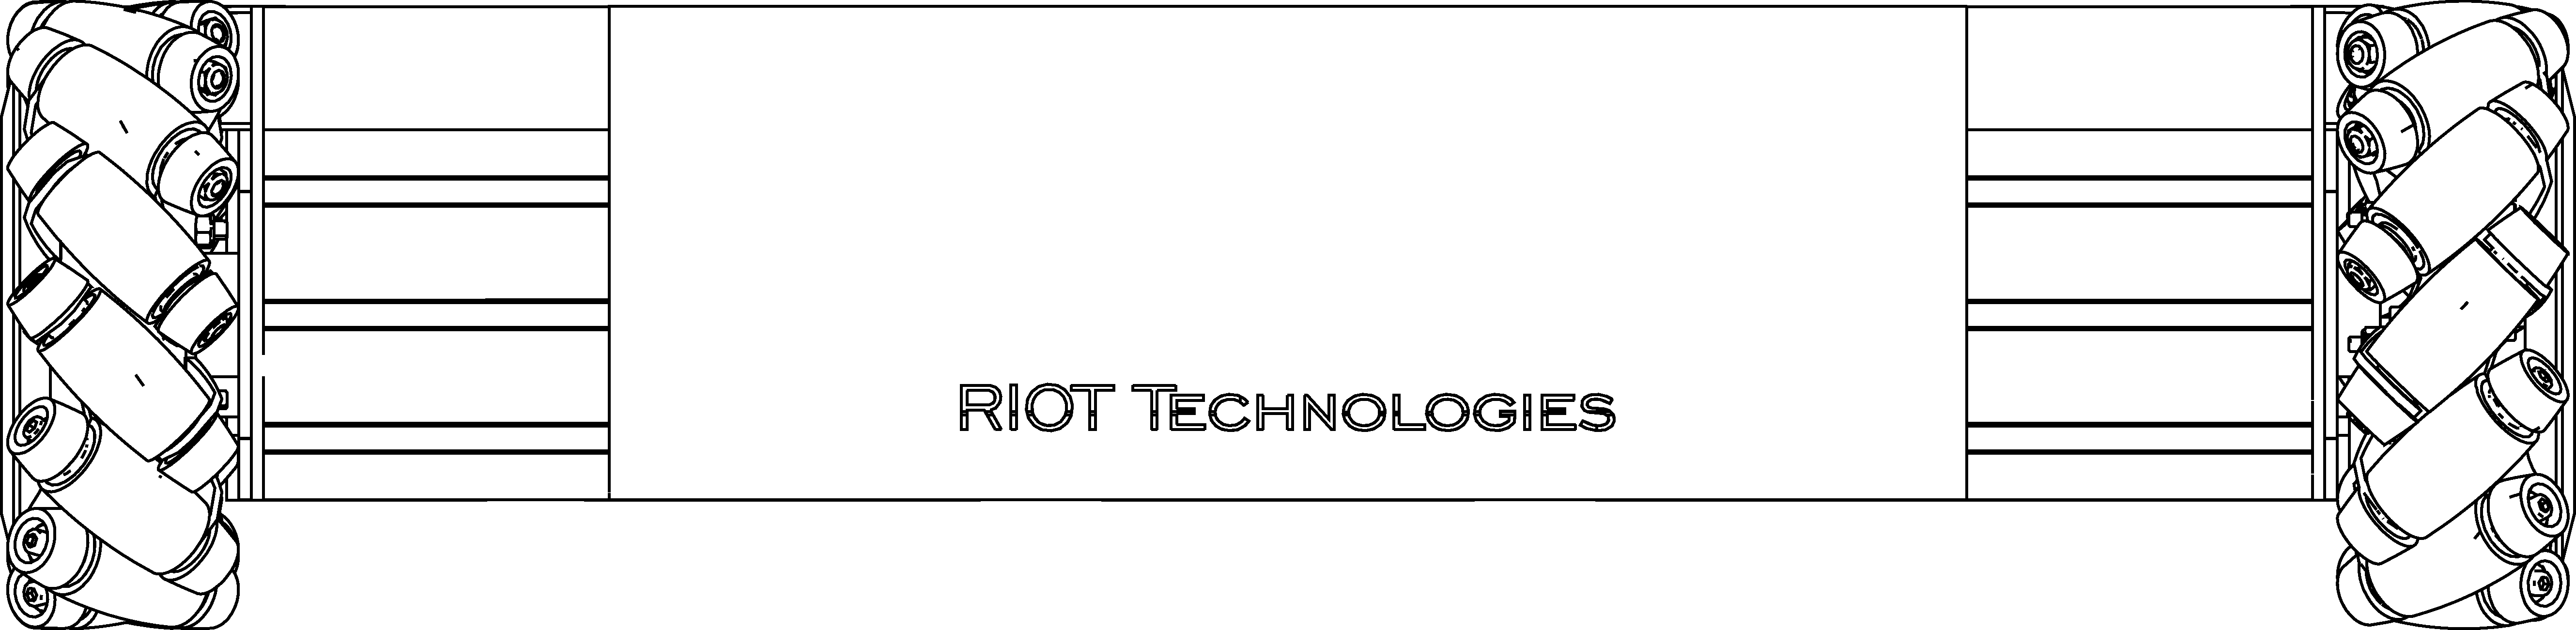
\includegraphics[width=0.5\textwidth]{graphics/base_front.pdf}
	\caption{Platforma mobilna --- widok z tyłu.}
	\label{fig:base_front}
	\end{figure} 

	Platforma posiada 3 stopnie swobody. 
	\begin{itemize}
		\item Ruch bez obrotu równolegle do osi X.
		\item Ruch bez obrotu równolegle do osi Y.
		\item Obrót w płaszczyźnie podłoża.
	\end{itemize}

\section{Koła szwedzkie}
	Koła szwedzkie, zwane także kołami Mecanum, to specjalne koła z dodatkowymi rolkami na obwodzie, ustawionymi pod kątem $45^\circ$ do osi koła.
	Rolki są pasywne i obracają się niezależnie od siebie. Każde koło ma 12 takich rolek, patrz rysunek \ref{fig:wheel}.
	W platformie ich osie ustawione są w ten sposób, że osie najwyższych, lub najniższych, rolek dwóch kół z tej samej strony robota przecinają się pod kątem prostym.
	Innymi słowy, robot ma identycznie ustawione koła na przeciwległych wierzchołkach, i razem ustawione są w kształt litery \emph{X}, patrząc na nie z góry.
	Warto pamiętać, iż oś aktualnie dolnej rolki jest prostopadła do osi górnej rolki.

	Istnieje również odwrotna odmiana ustawienia kół, w której rolki tworzą literę \emph{O}, 
	czyli oś przednia jest zamieniona z tylną, lub jakby cała platforma była odwrócona do góry nogami.
	Ten drugi sposób także pozwala na ruch wielokierunkowy, ale nie jest tak często stosowany \cite{paletobot}.

	\begin{figure}[H]
	\centering
	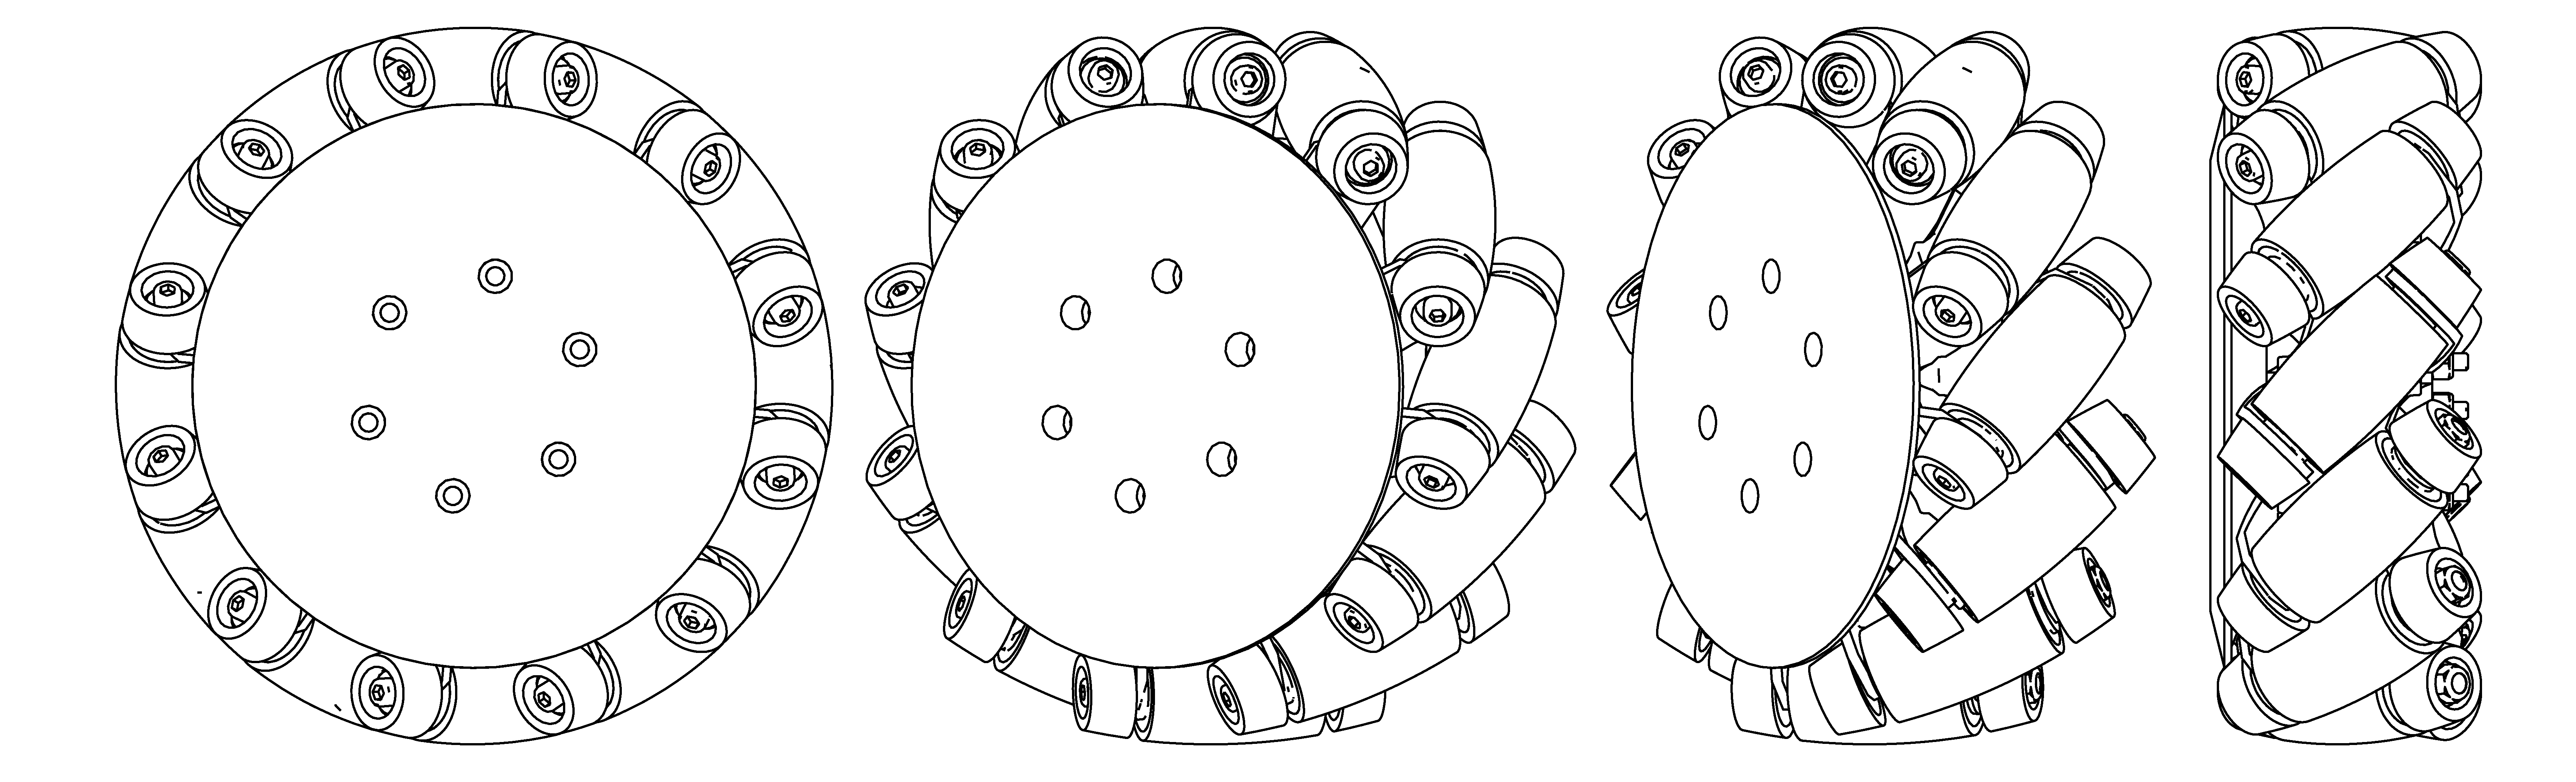
\includegraphics[width=\textwidth]{graphics/wheel.pdf}
	\caption{Widok 12 rolkowego koła szwedzkiego opisywanej platformy wielokierunkowej.}
	\label{fig:wheel}
	\end{figure} 

	Każde koło ma 3 stopnie swobody \cite{kinematic_modeling}, tak samo jak cała platforma.
	\begin{itemize}
		\item Obrót koła w osi.
		\item Rotacje pojedynczych rolek.
		\item Poślizg obrotowy w miejscu styku rolki z podłożem.
	\end{itemize}

	Na podstawie rysunku \ref{fig:wheel} widać, że krzywizna rolki jest tak ustawiona, aby punkt kontaktu rolki z podłożem w czasie obrotu płynnie przechodził na następną rolkę.
	Celem jest utrzymanie równej odległości osi od płaszczyzny podłoża.
	Nie powinno być efektu przeskoku z jednej rolki na drugą, gdyż to wprowadza nierówne tarcie, losowe poślizgi i nadmierne zużycie elementów wykonawczych.
	Kształt pojedynczej rolki zawiera się w paraboloidzie, wzory opisujące kształt rolki są złożone.
	Zazwyczaj przybliża się taką rolkę wycinkiem torusa, w celu uproszczenia produkcji \cite{rollers}.

	Istnieją także inne budowy kół, złożone z wielu małych rolek, tak aby w każdym momencie więcej jak jedna rolka dotykała podłoża.
	Można także złożyć kilka powyższych kół obok siebie w jedno koło.
	Przydatne jest to dla robotów transportujących duże masy, gdyż zmniejsza to obciążenie pojedynczych rolek.
	Niestety, taka budowa jest chroniona aktywnym patentem, więc pojedyncze koło, na które patent już wygasł, jest jedynym popularnie używanym \cite{paletobot}.

	Podstawowym problemem technologicznym koła jest nie tylko skomplikowana budowa, ale także ślizganie się rolek po powierzchni.
	Odległość osi od płaszczyzny nieznacznie zmienia się przy przenoszeniu ciężaru z rolki na rolkę, co przy dużych prędkościach powoduje drgania i jeszcze większe błędy pomiarów.
	Środkowy przegub zmniejsza ich przenoszenie na drugą część platformy.
	Poślizg kół powoduje, że enkodery nie mogą być jedynymi czujnikami służącymi do wyznaczania pozycji bazy, gdyż są zbyt mało dokładne \cite{heavy}.
	
	Dodano więc dwa czujniki laserowe, opisane dokładniej w sekcji \ref{sec:lidar}, aby program sterujący nie bazował jedynie na odometrii przy 
	wyznaczaniu sterowania. Istnieje także czujnik inercji, wykrywający zmianę rotacji i prędkość kątową robota.
	%TODO referencja

	\subsection{Działanie platformy}
	Standardowe koło, używając tarcia, przekształca prędkość kątową na liniową w płaszczyźnie obrotu. 
	Specjalne koło Mecanum ma dodatkowy wektor, równoległy do osi obrotu, 
	zatem prędkość wypadkowa jest obrócona o 45° w stosunku do wektora prędkości standardowego koła, 
	zależnie od typu koła (prawoskrętne lub lewoskrętne) i kierunku obrotu.

	\begin{figure}[H]
	\centering
	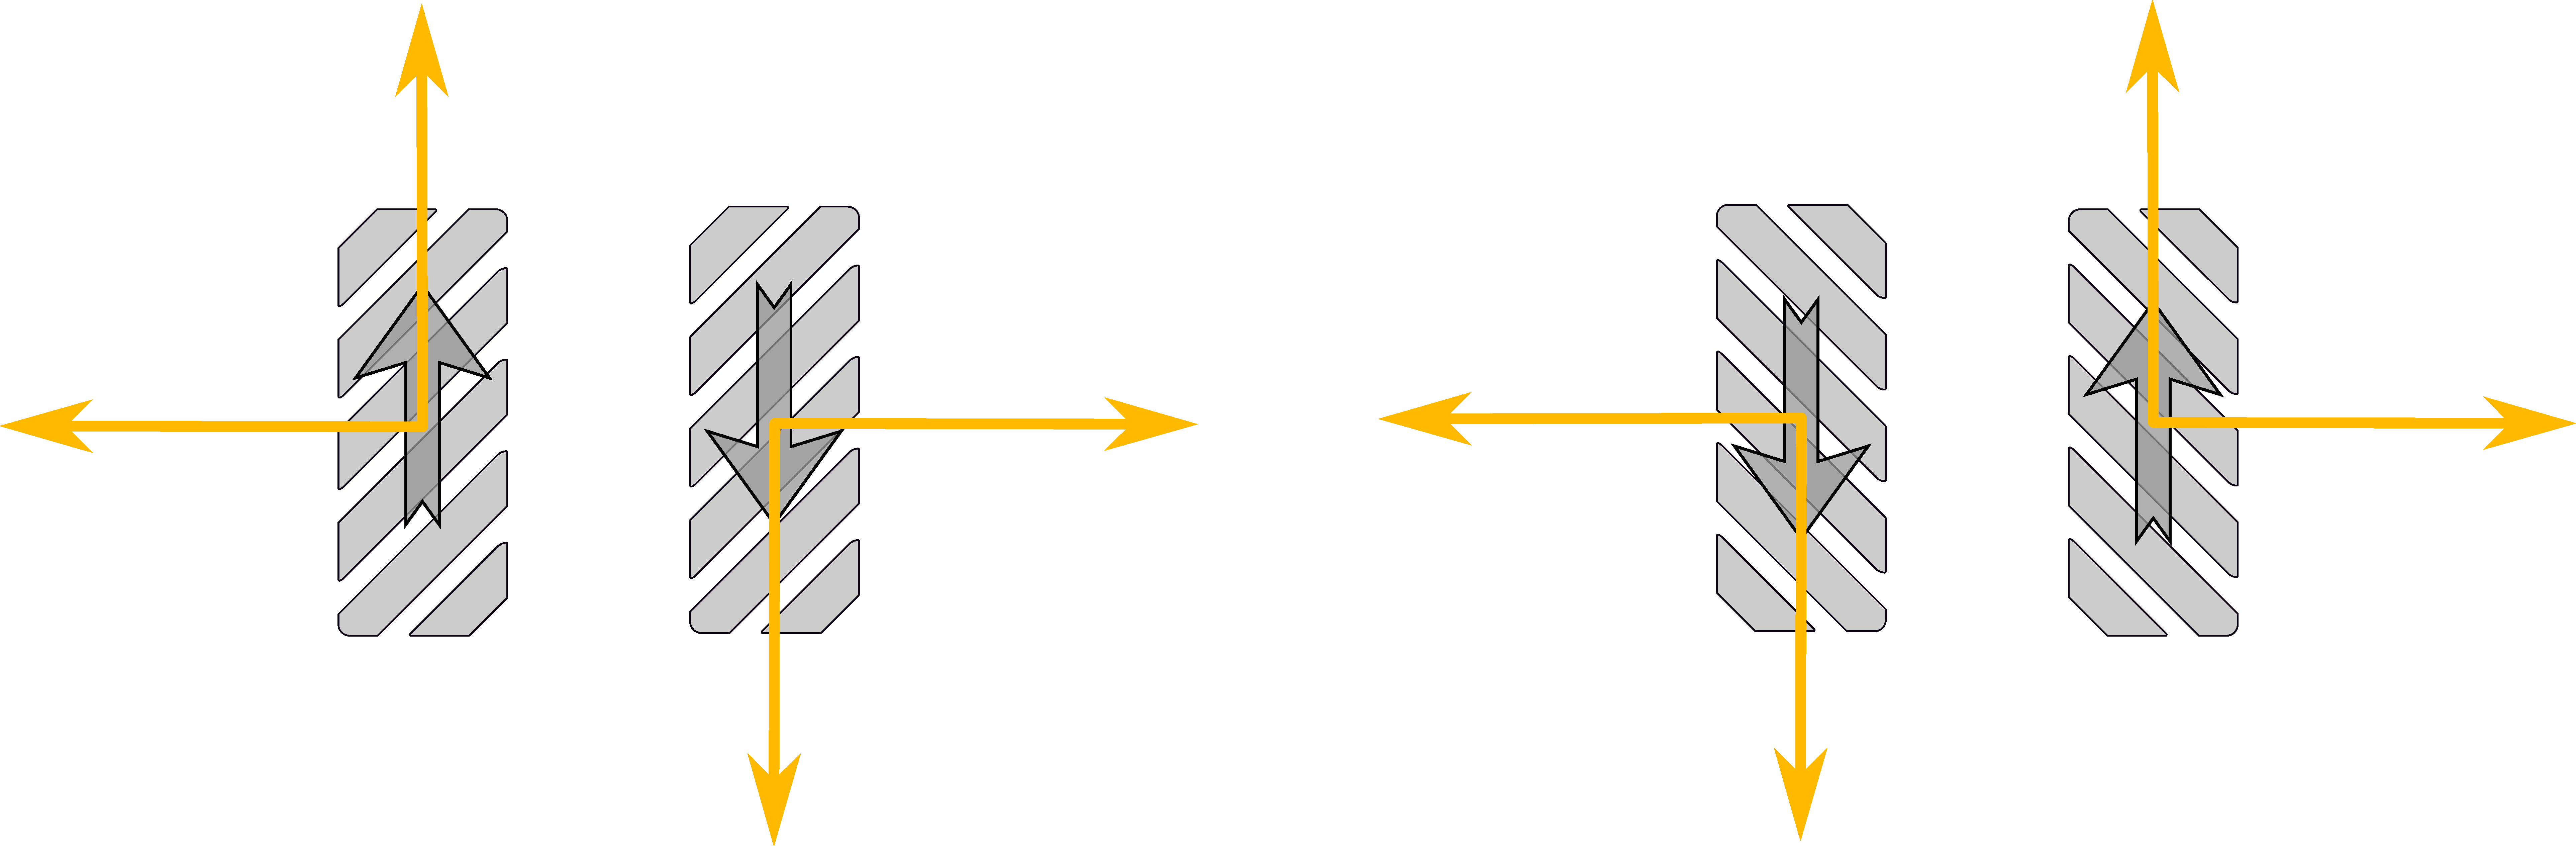
\includegraphics[width=\textwidth]{graphics/vectors.pdf}
	\caption{Wektory składowe i wypadkowe koła widzianego z góry.}
	\label{fig:wheel_vectors}
	\end{figure} 

	Ustawiając te koła w odpowiedni, opisany wcześniej na obrazku \ref{fig:base_top}, sposób, można wywołać odpowiednie znoszenie się składowych prędkości,
	a w efekcie pozwolić robotowi na poruszanie się w kierunkach nieosiągalnych dla pojazdów o standardowych kołach.
	Warto nałożyć te składowe na wcześniejszy rysunek \ref{fig:mecanum_dirs}, aby dokładniej zobaczyć, 
	dlaczego koła nadają platformie daną prędkość wypadkową przy odpowiednim obrocie kół.

	\begin{figure}[H]
	\centering
	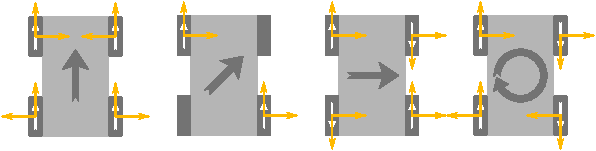
\includegraphics[width=\textwidth]{graphics/mecanum_dirs_vect.pdf}
	\caption{Ruchy platformy widzianej z góry, z nałożonymi składowymi wektorów prędkości. Ciemniejszym kolorem zaznaczono znoszące się składowe.}
	\label{fig:mecanum_dirs_vect}
	\end{figure} 

	Warto rozpatrzyć każdy przypadek. Platforma posiada jedną płaszczyznę symetrii, ze względu na asymetryczny przegub.
	\begin{enumerate}
		\item Wektory o kierunku prostopadłym do pionowej płaszczyzny symetrii urządzenia znoszą się, pomimo że mają przeciwne zwroty na przedniej i tylnej parze kół.
		Pozostają jedynie składowe równoległe do płaszczyzny symetrii, które powodują prostoliniowy ruch naprzód.
		\item Dwa koła nie obracają się. Nie jest to ruch pasywny, gdyż taki wprowadzałby nieprzewidywane poślizgi, a aktywne hamowanie.
		Wektory się nie znoszą i platforma wykonuje ruch pod kątem 45° do płaszczyzny symetrii.
		\item Ruch podobny jest do przypadku 1. Tutaj również wektory znoszą się parami, jednak tym razem na prawych kołach i lewych. 
		Pozostają składowe prostopadłe do płaszczyzny symetrii.
		\item Prędkość kątowa powstaje, gdy wypadkowa kół po jednej stronie platformy znosi się z wypadkową po drugiej stronie.
	\end{enumerate}

	Warto nadmienić, że gdy wypadkowy wektor prędkości koła jest prostopadły do osi koła, to jest gdy
	koło porusza się zgodnie z kierunkiem obrotu, w idealnym przypadku rolki nie obracają się.
	Inaczej mówiąc, rolka będzie się obracać tym mocniej, im bardziej ruch koła wymuszany jest równolegle do osi koła, 
	czy to na skutek znoszenia się wektorów, czy oporu przeszkody.
	
	Przykładowo, przy ruchu naprzód rolki koła się nie obracają, lecz przy ruchu w bok biorą aktywny udział.
	Ma to wpływ na zużywanie się tych elementów, nie tylko z punktu widzenia ilości obrotów danej rolki na pokonanym dystansie, 
	ale także sposobu w jaki wymuszany jest jej ruch.
	Rolki robota przy jeździe zawsze obracają się szarpanym ruchem w obie strony, ze względu na poślizgi od innych kół, 
	niejednostajne tarcie piast wszystkich rolek, czy różnice terenu. 
	Zatem przejazd przykładowego odcinka, przy platformie ustawionej przodem do kierunku jazdy, lub bokiem, będzie w różnym stopniu i w różny sposób zużywał elementy wykonawcze robota.
	To, jak dokładnie zużywają się przeguby i jaki styl jazdy opłaca się zastosować, aby zminimalizować uszkodzenia elementów jest dużą, odrębną dziedziną nauki.
	Odpowiednio skomplikowany algorytm sterowania może brać pod uwagę tą mechanikę kół.

\section{Czujnik laserowy}
	\label{sec:lidar}
	Program sterujący platformą nie jest w stanie dokładnie określić pozycji robota, bazując jedynie na odometrii.
	Potrzebny jest zatem czujnik laserowy.
	Platforma wyposażona jest w dwa, dwuwymiarowe czujniki typu LiDAR firmy SICK.
	LiDAR to zbitek wyrazów \emph{light} i \emph{radar}, chociaż skrót może być rozwinięty w różne słowa.

	\begin{figure}[H]
	\centering
	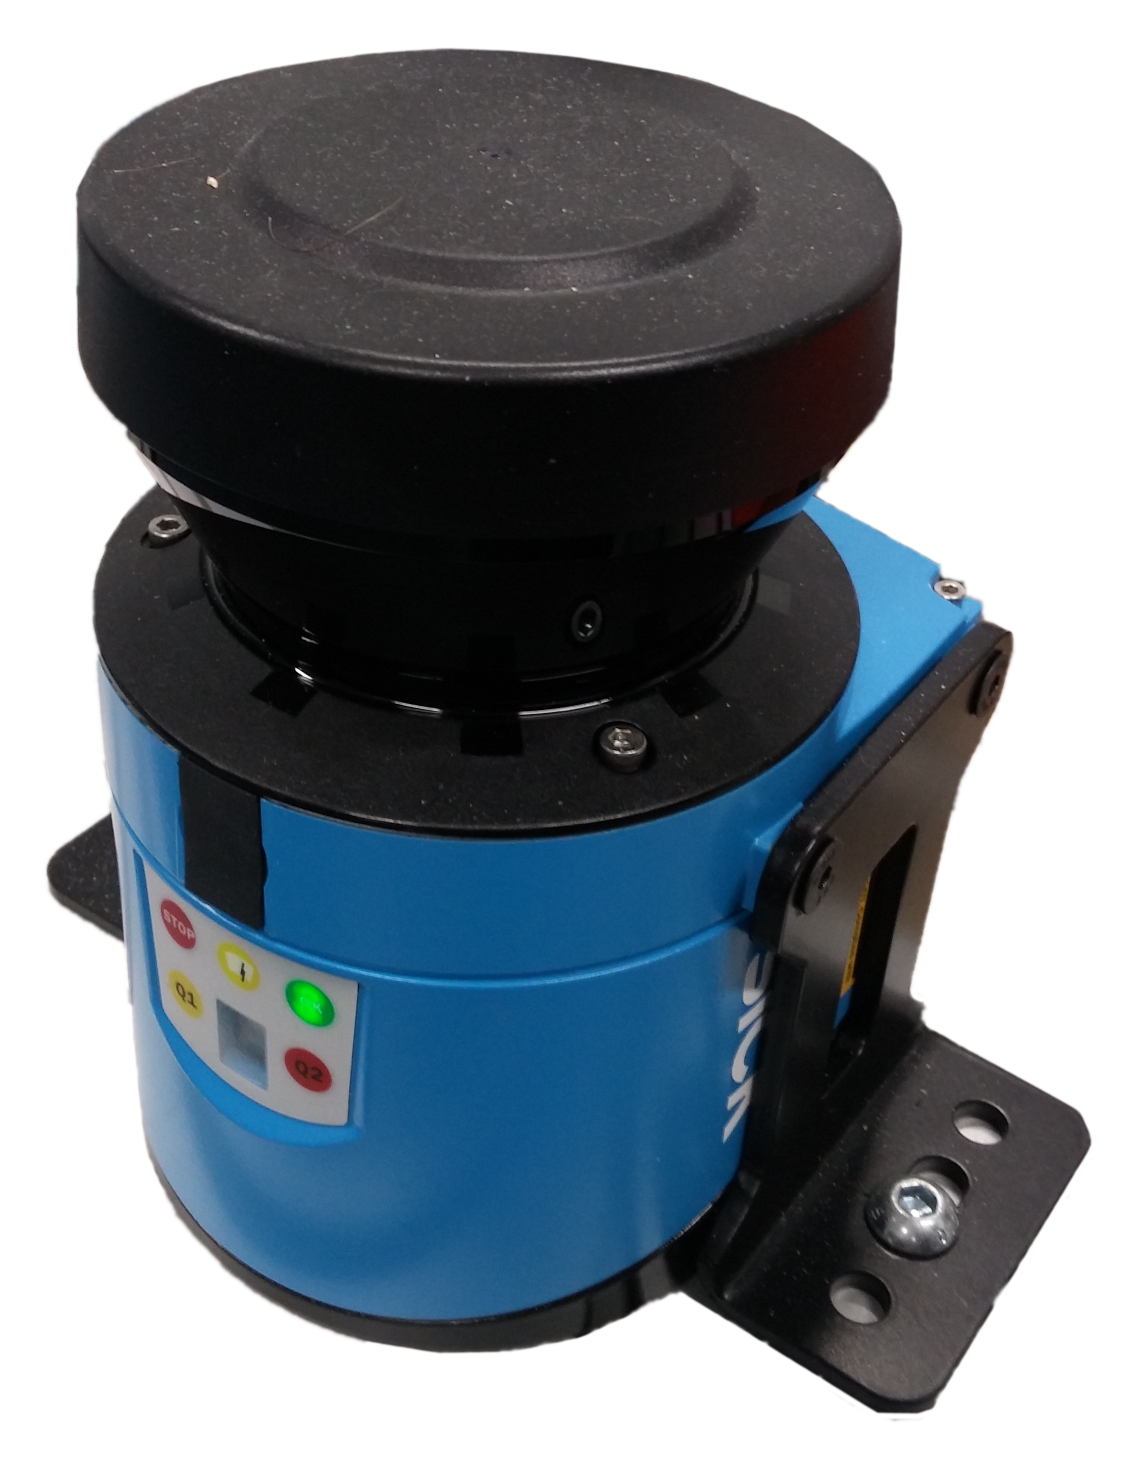
\includegraphics[width=0.5\textwidth]{graphics/sensor.png}
	\caption{Czujnik laserowy SICK LMS100-10000.}
	\label{fig:sensor}
	\end{figure} 

	\subsection{Zasada działania}
		Wszystkie czujniki tego typu mają bardzo podobną zasadę działania.
		W środku urządzenia znajduje się obrotowe lusterko, zwrócone pod kątem 45° do osi obrotu.
		Równolegle do osi jego obrotu znajduje się laser, który emituje pulsacyjną wiązkę podczerwonego promienia co pewien okres czasu.
		Emitowanie stałego promienia może być niebezpieczne dla wzroku obsługujących go ludzi.
		Aktualna pozycja lusterka jest wykrywana przez enkoder.
		Obok lasera jest czujnik, który bada wysłane przez laser, odbite od lusterka, obiektu i ponownie lusterka, światło.

		Na koniec, algorytm we wbudowanym mikrokontrolerze ustala kąt i odległość czujnika od wykrytego obiektu.
		Odpowiada także za usunięcie szumu i ewentualnych odbić promienia.
		Komunikacja z urządzeniem może odbywać się za pomocą różnych interfejsów sieciowych, zazwyczaj w architekturze typu master-slave.
		W przypadku tej platformy na obecny czas jest to Ethernet.
		
		Skośna szyba, będąca wycinkiem powierzchni stożka, zabezpiecza wnętrze przed zanieczyszczeniami, jej kształt niweluje ewentualne odbicia lasera, emitowanego poziomo ze środka.
		W niektórych czujnikach montuje się także szereg dodatkowych diod podczerwieni na obrębie szyby, skierowanych w górę, lub w dół, oraz czujniki/reflektory z drugiej strony.
		Pozwala to na wykrycie stopnia zanieczyszczenia szyby, aby powiadomić użytkownika o potrzebie wyczyszczenia urządzenia.

	\subsection{Komunikacja}
		Wysyłając do czujnika odpowiedni ciąg bajtów, można ustawić jego tryb działania, odpytać o zebrane dane, czy wykryć konfigurację i stan.

		W przypadku tej platformy, komunikacja odbywa się poprzez interfejsy EtherCAT i Ethernet.
		EtherCAT to sposób komunikacji urządzeń po kablu Ethernetowym, w trybie \emph{master}-\emph{slave}, przy zachowaniu sztywnych ram czasowych. 
		\emph{Master} wysyła pakiet do podłączonych szeregowo urządzeń \emph{slave}, które przekazują go przez siebie i w razie potrzeby modyfikują dane w locie.
		
		Program odbierający dane od czujnika komunikuje się bezpośrednio z urządzeniem, które zwraca pakiety zawierające pomiary z ostatniego obrotu czujnika, oraz dodatkowe dane 
		opisujące sam pomiar, takie jak czas, początkowy kąt pomiaru, czy tryb pacy.
		Dokładne pola w pakiecie i cechy czujnika dostępne są na stronie producenta \cite{sick_website}.

		Urządzenie wspiera uwierzytelnianie przez hasło, wgrywanie nowego oprogramowania,
		ustawienia czasu, oraz zmianę różnych parametrów działania.

	\subsection{Podstawowe cechy}
		Czujnik składa się z dwóch części, głównego trzonu, oraz nakładki.
		Połączenie tych elementów powoduje, że jego zakres pomiaru posiada martwy kąt.
		Przedstawia to dobrze grafika producenta \ref{fig:lidar}.
		\begin{figure}[H]
		\centering
		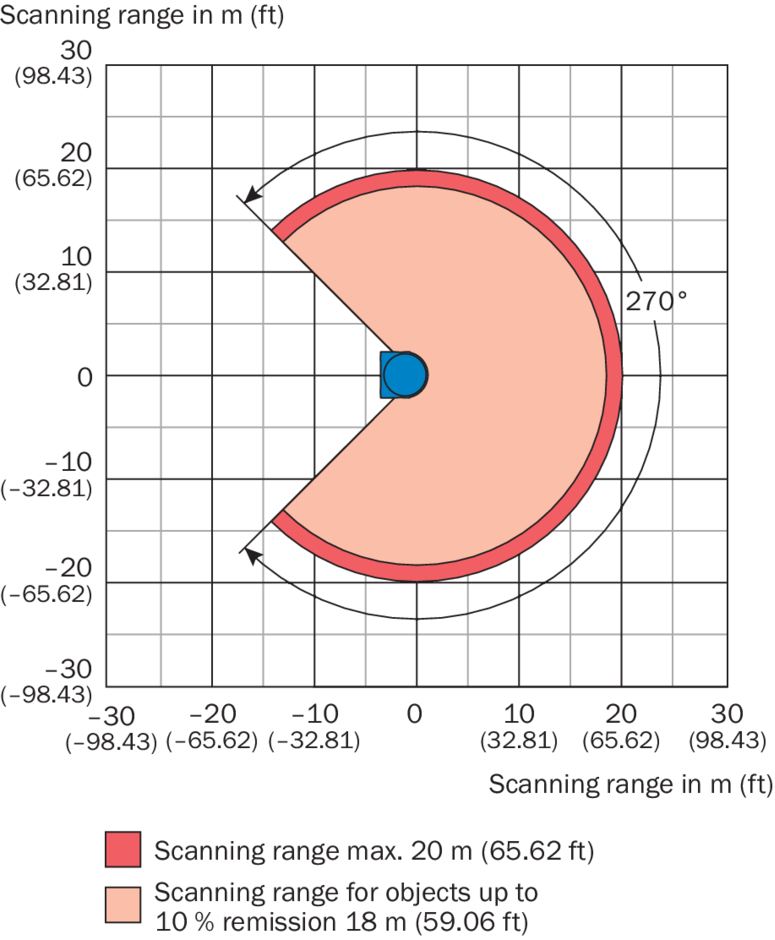
\includegraphics[width=0.6\textwidth]{graphics/sick.png}
		\caption{Wykres producenta dotyczący zasięgu czujnika.}
		\label{fig:lidar}
		\end{figure} 
		
		\begin{table}
		\centering
		\begin{tabular}{l r}
		Cecha & Wartość \\
		\hline
		Kąt pracy & 270\textdegree \\
		Długość fali światła lasera & 905 nm (podczerwień) \\
		Częstotliwości skanowania & 25 Hz / 50 Hz \\
		Maksymalna odległość obiektu & $\approx$ 20 m \\
		Rozdzielczość kątowa & $0,25 \degree$ / $0,5 \degree $ \\
		Systematyczny błąd pomiarowy & $\pm 0,03$ m \\
		Przypadkowy błąd odległości & $0,012$ m \\
		\end{tabular}
		\caption{Podstawowe cechy czujnika laserowego.}
		\label{tab:lidar}
		\end{table}
		Na podstawie tych danych można obliczyć, że w jednym przebiegu po całym zakresie kątowym urządzenia, 
		emitowane jest około 1080, lub 540 impulsów (w zależności od trybu działania).
		Taka ilość promieni wymagana jest w symulacji, aby wiernie odwzorować urządzenie.

\section{Czujnik inercji}
	Ten czujnik to małe urządzenie, posiadające zazwyczaj zestaw wewnętrznych czujników, przydatnych przy określaniu prędkości, rotacji i przyspieszeń modułu.
	Dodatkowo, wiele zestawów tego typu posiada także czujniki pola magnetycznego, położenia, lub nawet termometry.
	
	Czujnik użyty w platformie to ADIS16460AMLZ, firmy Analog Devices. Szczegółowa dokumentacja jest dostępna na stronie producenta \cite{adis_website}.
	
	Urządzenie ma kształt małej kostki i komunikuje się za pomocą złącza SPI, a co za tym idzie, wymaga zewnętrznego mikrokontrolera, aby móc wysyłać wygenerowane dane
	do sieci do innych urządzeń.
	
	Czujnik posiada:
	\begin{itemize}
		\item Trzyosiowy żyroskop.
		\item Trzyosiowy akcelerometr.
		\item Czujnik temperatury.
		\item Sprzętowe wspomaganie korekcji błędów i kalibracji.
	\end{itemize}
	
	Ten czujnik, podobnie jak opisany wcześniej LiDAR, również jest podatny na błędy pomiarowe, a co za tym idzie, należy dodać losowe odchylenia do generowanych danych.
	
	W symulacji nie jest używana informacja o temperaturze otoczenia, zatem nie ma potrzeby jej symulować.
